In the following section the experients from each theses to be tested are presented in a chronological manner.

\subsection{These 1 / Experiment 1}

The training of the network took around 11 days with a batchsize of 128 and $6.7\cdot10^5$ patches of size 32x32x32 voxels. The training was performced on 4 nvidia gtx 2080 ti and a initial learning rate of 10\textsuperscript{-4} decreasing by a factor of 10 as soon as the validation loss or the gamma pass rate on the validation set did not decrease for 50 epochs. The training was stopped when no improvement was observed at a learning rate of 10\textsuperscript{-6} for 50 epochs. 

The model reaches a mean gamma score of 96.16\% ± 6.12\% (median: 98.02\%) on the test dataset for prostate patients. (\autoref{fig:prediction}) shows a qualitative example of a target dose and the respective dose prediction and gamma map for a prostate cancer patient in the isocentric slice. 

\begin{figure}[h]
    \centering
    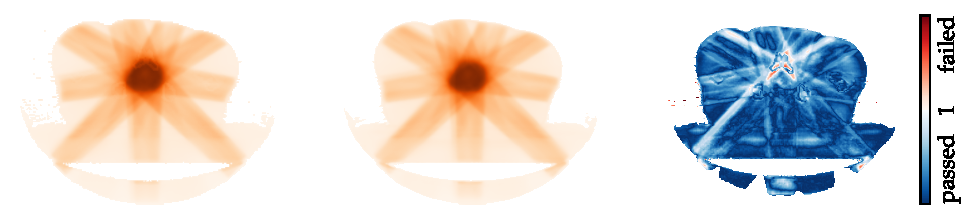
\includegraphics[width=\textwidth]{example.pdf}
    \caption{Dose prediction example on isocentric slice on prostate cancer patient from test cohort with prostate data only trained model. From left to right: target dose; dose prediction; gamma map for isocentric slice with a gamma pass rate of 98.02\%}
    \label{fig:prediction}
\end{figure}

\subsection{These 2 / Experiment 2}

Model performance for liver, mamma and head tumor sites are summarized in (table ...). 

\begin{table}[]
    \centering
    \begin{tabular}{|ll|cccc|}
    \hline
                            &                      & \textbf{Liver} & \textbf{Mamma} & \textbf{H\&N} & \textbf{LK} \\ \hline
    Number of Patient Plans & /1                   & 5              & 5              & 5             & 15          \\ \cline{1-2}
    Mean Gamma Passrate     & \multirow{3}{*}{/\%} & 77.69          & 63.25          & 76.19         & 82.12       \\
    STD Gamma Passrate      &                      & 10.13          & 6.72           & 4.99          & 11.51       \\
    Median Gamma Passrate   &                      & 80.39          & 63.48          & 77.67         & 85.9        \\ \hline
    \end{tabular}
    \caption{Summary of gamma passrates for liver, mamma, head and lyphnodes tumor patients}
    \label{tab:prost}
\end{table}


\subsection{These 3 / Experiment 3}

The training of the network took around 9 days with a batchsize of 128 and $5.0\cdot10^5$ patches of size 32x32x32 voxels. The training was performced on 4 nvidia gtx 2080 ti and a initial learning rate of 10\textsuperscript{-4} decreasing by a factor  10 as soon as the validation loss or the gamma pass rate on the validation set did not decrease for 50 epochs. The training was stopped when no improvement was observed at a learning rate of 10\textsuperscript{-6} for 50 epochs. 

Model performance for prostate, liver, mamma and head tumor sites are summarized in (table ...). 

\begin{table}[]
    \centering
    \begin{tabular}{|ll|C{1.4cm}C{1.4cm}C{1.4cm}C{1.4cm}C{1.4cm}|}
    \hline
                            &                      & \multicolumn{1}{l}{\textbf{Prostate}} & \textbf{Liver} & \textbf{Mamma} & \textbf{H\&N} & \textbf{LN} \\ \hline
    Number of Patient Plans & /1                   & 5                                     & 5              & 5              & 5             & 15          \\ \cline{1-2}
    Mean Gamma Passrate     & \multirow{3}{*}{/\%} & 97.85                                 & 97.59          & 87.46          & 90.68         & 90.71       \\
    STD Gamma Passrate      &                      & 2.82                                  & 4.56           & 6.61           & 6.4           & 9.6         \\
    Median Gamma Passrate   &                      & 98.59                                 & 99.92          & 86.15          & 92.74         & 94.19       \\ \hline
    \end{tabular}
    \caption{Summary of gamma passrates for liver, mamma, head and lyphnodes tumor patients}
    \label{tab:mixed}
\end{table}

A comparison between prostate only and mixed trained models is depictedd in fig. .... 

\begin{figure}[h]
    \centering
    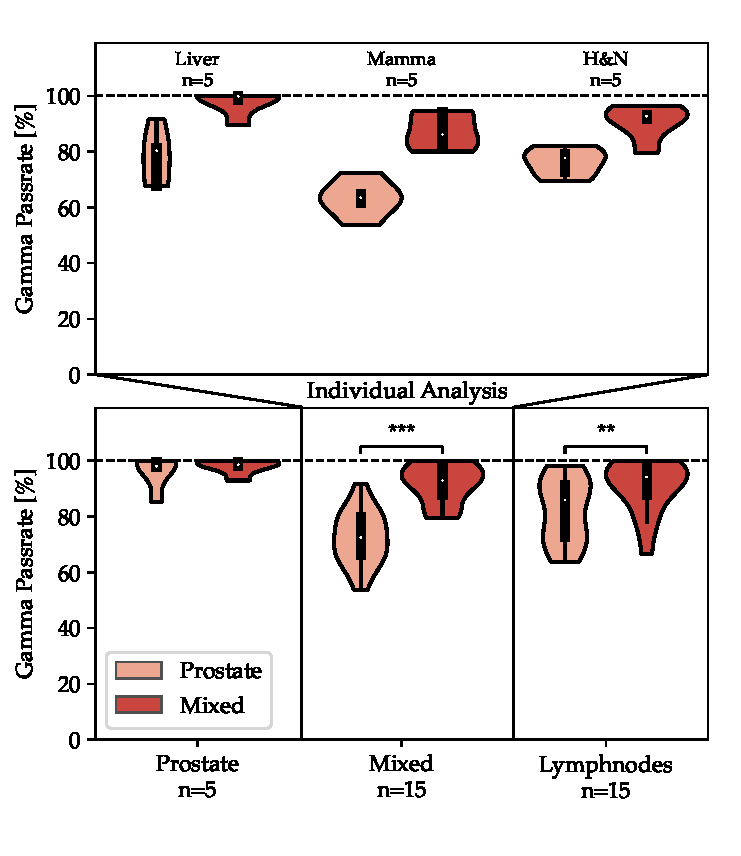
\includegraphics{plans.pdf}
    \caption{Prediction accuracy comparison between prostate only and mixed trained models. Passrates for liver, mamma and H\&N are combined into one group of `mixed' data. Significance level using a wilcoxon signed-ranked test are shown above the compared dataseries.}\label{fig:comparison}
\end{figure}

Single segment analysis gives a deeper insight into the actual performance differences of the model. we therefore assessed the gamma passrate for each single segment of all test data (fig ...). Additional information about performance regarding fieldsize can be benefitial to predict wether an unseen segment will reach high dose conformaty. fig ... shows the analysis for each segment of the test data regarding their fieldsize. additional information about the occurence of each discretized fieldsize range is shown in the background. 

\begin{figure}
    \centering
    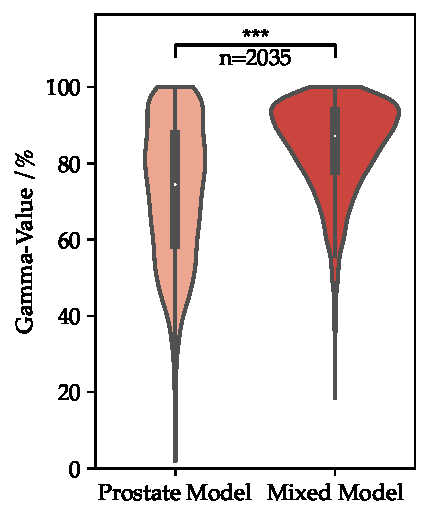
\includegraphics[width=0.4\textwidth]{segs_all.pdf}
    \caption{Prediction accuracy for all segments of the test data.}\label{fig:all_test}
\end{figure}

\begin{figure}
    \centering
    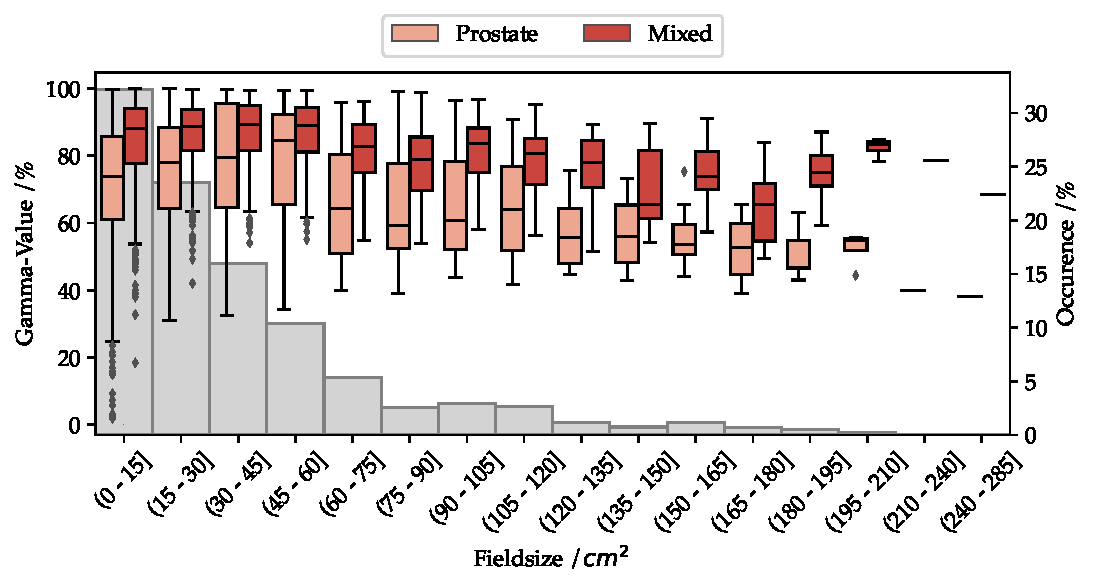
\includegraphics[width=\textwidth]{segs_fz_15.pdf}
    \caption{Prediction accuracy of each segment with allocation in terms of field size for prostate only and mixed trained model.}\label{fig:fz_test}
\end{figure}

\subsection{These 4 / Experiment 4}